\documentclass[thesis]{RyanPoster}
\usepackage{graphicx}
\usepackage{natbib}
\usepackage{booktabs}
\usepackage{subfig}
\usepackage{amsmath}
\usepackage{textcomp}
\usepackage{url}
\usepackage[english]{babel}

\author{Ryan Desfosses, Julie Ziffer, Matt Walker, Derick Arel, Tom Harvell}
\title{Using AutoClass Artificial Intelligence Program to Classify SDSS and IRAS Asteroidal Data}

\begin{document}
\begin{poster}

\section{Current Asteroid Classification}

\begin{center}
\begin{tabular}{ | p{23cm} | p{23cm} | }
\hline
\large{\bf Tholen Classification (1984)} & \large{\bf SMASS Clasification (2002)} \\ \hline\hline
A widely used taxonomy & More recent, higher resolution (no albedo considered).  \\ \hline
Based on spectroscopic measurements from Eight-Color Asteroid Survey (ECAS) & Based on the Small Main-Belt Asteroid Spectroscopic Survey (SMASS) \\ \hline
Original formulation based on 978 asteroids & Survey included 1447 asteroids \\ \hline
14 types with majority falling into 1 of 3 categories: & 24 types in three main categories: \\
\hspace{15} C-group: dark carbonaceous objects & \hspace{15} C-group: carbonaceous objects \\
\hspace{15} S-type: silicate (stony) objects & \hspace{15} S-group: silicate (stony) objects \\
\hspace{15} X-group: metallic objects & \hspace{15} X-group: metallic \\
\hline
\end{tabular}
\end{center}

\section{The Problem}%
With over 530,000 known asteroids the current classification system represents a data sample of less than 1\% of the known population.

The huge size of existing data sets make it difficult or impossible to organize the available information in any useful way using traditional plotting and/or classification methods.

\section{Relevance}
Information obtained about asteroid stratification may help us better understand the processes by which the solar system was formed.  

Part of NASA's 2010 Science Mission Directorate:
Goal: "Ascertain the content, origin, and evolution of the solar system, and the potential for life elsewhere."
Among the fundamental questions:
What is the inventory of solar system objects and what processes are active in and among them?
What are characteristics of small bodies and planetary environments that pose hazards and/or provide resources?

\section{Autoclass}%
AutoClass essentially makes a guess, H, about the
possible classes and its degree of belief, P(H), in H. 
Each class described in H has a distribution of possible values for each attribute. AutoClass then begins to analyze the input attributes and comes up with some arrangement of them, E, based on the likelihood functions for each attribute (determined by the models chosen). From there a likelihood function L(E—H) is developed which describes the likelihood of some particular attribute arrangement, E,
given the current guess, H. The joint probability
J(EH)=L(E—H)*P(H), divided by the sum of J(EH)
for all possible H is called posterior degree of belief,
P(H—E), in H given E. What we have is the degree
of belief in H given a set of evidence E, Bayes’ Rule,
describing how beliefs should change with evidence.
By repeating this process over many guesses, AutoClass determines the most probable H. This is the
classification.

\begin{figure}
\begin{center}
\fbox{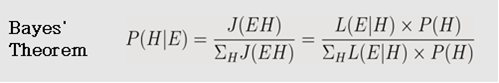
\includegraphics[width=14in]{images/Bayes.png}}
\caption{Formula for Bayesian Theory}%
\end{center}
\end{figure}

\vfill
\columnbreak
\section{Kirkwood Gap}
\begin{figure}
\begin{center}
\fbox{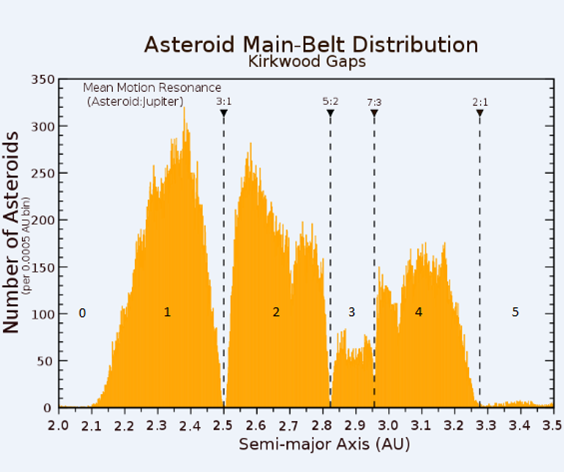
\includegraphics[width=10in]{images/Kirkwood.png}}
\caption{The Kirkwood Gaps are the vacant regions in the asteroid belt that are formed by Jupiter's gravitational effect }%
\end{center}
\end{figure}

\begin{figure}
\begin{center}
\fbox{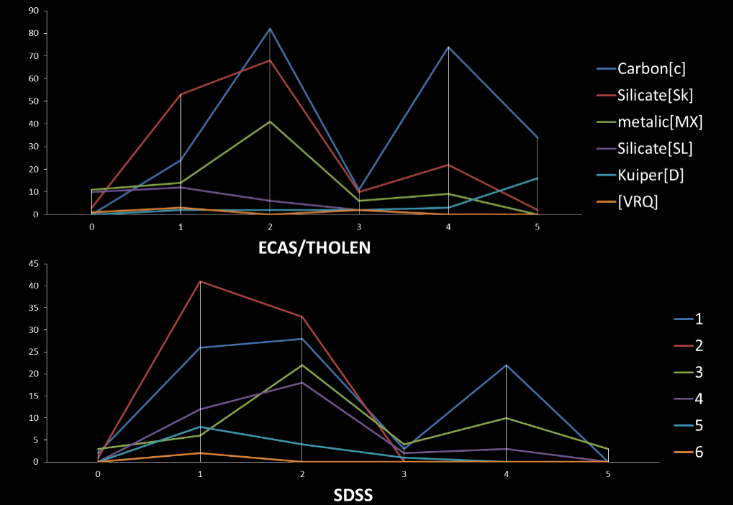
\includegraphics[width=10in]{images/sdss.png}}
\caption{Top: The same technique was applied with ECAS and IRAS albedos.  The distribution of the different classes throughout the Kirkwood regions of the asteroid belt.  Bottom: 257 SDSS objects (not including albedos) and their distribution throughout the Kirkwood regions. }%
\end{center}
\end{figure}

\begin{figure}
\begin{center}
\fbox{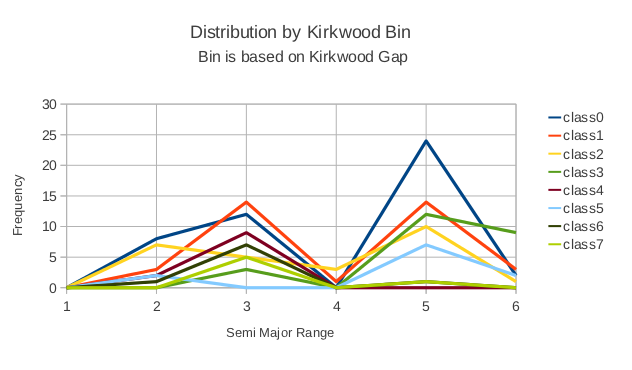
\includegraphics[width=10in]{images/KirkwoodBin.png}}
\caption{The graph above shows the regions for which the asteroids in SDSS and with IRAS albedos reside}%
\end{center}
\end{figure}

\section{Results}
Our most interesting findings were unexpected: the albedos were labeled the least important factor.  Upon examining the data, we found that the majority of the asteroids had relatively large semi-major axes.  Since outer-belt asteroids are often primitive in nature with correspondingly low albedo, the majority of our asteroids likely have similar low albedo.  The one class that has a moderately high albedo influence was the group with a shorter semi-major axis.  Due to our success with these smaller data sets, we are optimistic about Autoclass's ability to classify asteroids in SDSS and other large databases.  

\end{poster}
\end{document}
